In this task, we apply bifurcation theory to the SIR model, a commonly used framework in epidemiology for understanding the spread of diseases within a population. The model categorizes the population into three compartments: Susceptible (S), Infected (I), and Recovered (R). Individuals in the susceptible category can contract the disease, becoming infected, and those who are infected will eventually recover, gaining immunity. The transitions between these compartments are governed by a set of differential equations that determine the rate of movement from one compartment to another. Parameters such as the rate of infection and recovery are pivotal in comprehending the disease's spread and how it can be controlled.

\begin{itemize}
\item \textbf{Part 1,2: Implementation of the SIR Model}
To address the task at hand, we have updated the existing \texttt{sir\_model.py} file to include the missing imports and also equations. So we have successfully implemented the SIR model. The model is characterized by the following system of differential equations:

\begin{align}
\frac{dS}{dt} &= A - \delta S - \frac{\beta SI}{S + I + R}, \\
\frac{dI}{dt} &= -(\delta + \nu)I + \frac{\beta SI}{S + I + R} - \mu(b, I)I, \\
\frac{dR}{dt} &= \mu(b, I)I - \delta R.
\end{align}

In these equations, \( S \), \( I \), and \( R \) denote the susceptible, infected, and recovered populations, respectively. The parameters include the recruitment rate \( A \), the natural death rate \( \delta \), the disease-induced death rate \( \nu \), the contact rate \( \beta \), and the recovery rate \( \mu \). The recovery rate \( \mu \) is a function of the infected population \( I \) and the number of beds per 10,000 individuals \( b \), defined as:

\begin{equation}
\mu(b, I) = \mu_0 + \frac{(\mu_1 - \mu_0)b}{b + I}.
\end{equation}

For our simulation, we set the initial time \( t_0 \) to the end time \( t_{\text{end}} \) of 1000. The SIR model parameters were chosen as follows: \( \beta = 11.5 \), \( A = 20 \), \( \delta = 0.1 \), \( \nu = 1 \), \( b = 0.01 \) (representing the bed parameter), \( \mu_0 = 10 \) (minimum recovery rate), and \( \mu_1 = 10.45 \) (maximum recovery rate).

% Figure \ref{fig:task5a} visualizes the dynamics of the SIR model over time in three different plots which we will describe in the following. 

\begin{itemize}
\item{Population Dynamics}


\begin{figure}[H]
    \centering
    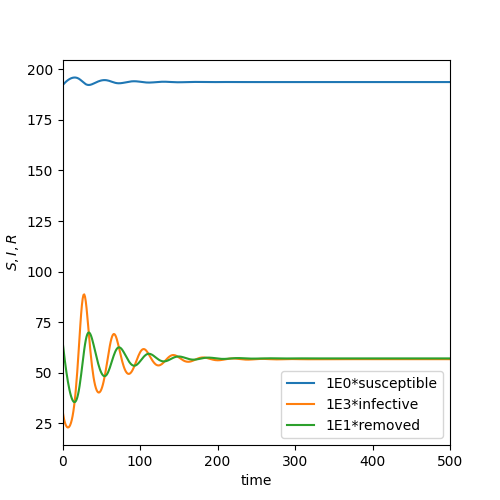
\includegraphics[width=0.4\textwidth]{images/task5/ex4_t5_1a.png}
    \caption{Population dynamics over time}
    \label{fig:task5_1a}
\end{figure}


The first plot (figure \ref{fig:task5_1a}) details the time evolution of the populations:
    \begin{itemize}
        \item The blue line illustrates the susceptible population ($S$), scaled by $1 \times 10^0$.
        \item The orange line traces the infected population ($I$), scaled by $1 \times 10^3$.
        \item The green line represents the recovered population ($R$), scaled by $1 \times 10^1$.
    \end{itemize}

Time evolution of a SIR model for disease spread. The blue curve represents the number of susceptible individuals ($10 \times S$), decreasing over time as they become infected. The orange curve illustrates the number of infectious individuals ($10^3 \times I$), initially rising and then falling as the disease progresses. The green curve shows the number of removed individuals ($10 \times R$), including those who have recovered or died, which increases over time. The susceptible population declines without fluctuation, while the infected population shows a rise followed by a decline, and the removed population consistently increases, indicating the progression of recovery or mortality due to the infection.



\item {Recovery Rate and Infected Population}

\begin{figure}[H]
    \centering
    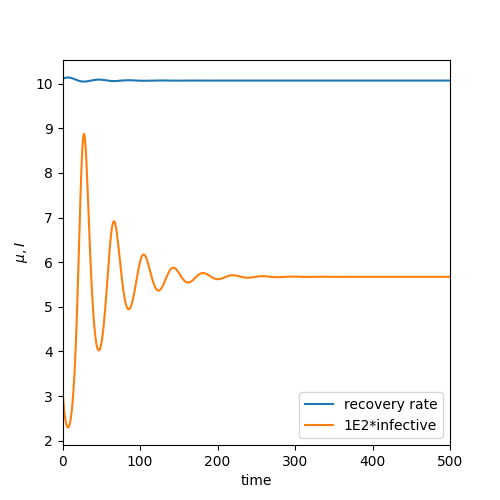
\includegraphics[width=0.4\textwidth]{images/task5/ex4_t5_1b.png}
    \caption{Recovery rate and infected population}
    \label{fig:task5_1b}
\end{figure}

The second graph (figure \ref{fig:task5_1b}) illustrates both the recovery rate ($\mu$) and the infected population:
    \begin{itemize}
        \item The blue line indicates the recovery rate, which exhibits relative constancy over the observed period.
        \item The orange line represents the infected population ($I$), multiplied by 100 ($100 \times I$), and shows fluctuating behavior with a general trend towards decrease. This is likely caused by the interplay between the fixed transmission rate ($\beta = 11.5$), the periodic recovery rate, and the stochastic initial conditions. The infection rate is determined by the contact rate, which is fixed, and the periodically varying recovery rate introduces non-linear dynamics into the system, resulting in the observed fluctuations. The model assumes a constant population with no births or deaths, except for those due to the disease.
    \end{itemize}
This graph illustrates the complex relationship between the recovery rate and the infected population, suggesting that the recovery rate does not depend solely on the infection numbers.


\item{Indicator Function}
\begin{figure}[H]
    \centering
    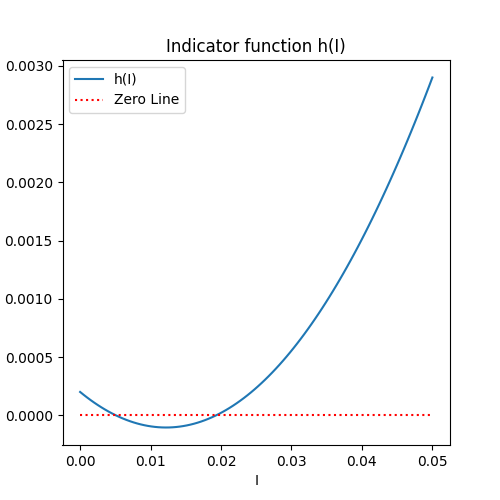
\includegraphics[width=0.5\textwidth]{images/task5/ex4_t5_1c.png}
    \caption{Indicator function h(I)}
    \label{fig:task5_1c}
\end{figure}
    
The third graph (figure \ref{fig:task5_1c}) features the indicator function $h(I)$ plotted against the infected population ($I$):
    \begin{itemize}
        \item The blue curve signifies the indicator function $h(I)$, utilized to identify bifurcation points or thresholds within the system.
    \end{itemize}
The indicator function is at zero for a range of $I$ values, which indicates a state of equilibrium. As the value of $I$ increases, $h(I)$ surges, indicating a possible bifurcation or a shift in the system's stability.

The reproduction number \( R_0 \) is calculated to be approximately 0.9957. The system is globally asymptotically stable if \( \beta \leq \delta + \nu + \mu_0 \); however, this condition is not met since the inequality evaluates to False. This implies that the system is not asymptotically stable.
\end{itemize}

\item \textbf{Part 3: Change of parameter b} \\
% Change b from 0.01 to 0.03 in small increments. What happens (from three starting points)?
We are set to modify the parameter 'b', which represents the number of beds, to observe a specific bifurcation phenomenon. To achieve this, we will adjust 'b' incrementally from 0.01 to 0.03, in steps of 0.001. This alteration will be applied across three different starting points for the populations: Susceptible (S0), Infected (I0), and Recovered (R0). The chosen initial conditions are (S0, I0, R0) = (195.3, 0.052, 4.4), (195.7, 0.03, 3.92), and (193, 0.08, 6.21). We show the results for the initial point (195.7,0.03,3.92) for our discussions in  fig \ref{fig:task5_3}.
\begin{itemize}
    \item \textbf{b$\textless$0.022:} For values of b less than 0.022, we observe the trajectories spiralling inwards towards a specific point over time. This spiralling signals that the populations of susceptible, infectious, and recovered individuals are stabilizing. This central point acts as an attractor, pulling the system towards a balanced state.
    \item \textbf{b=0.022:} At this value of b, we observe that the system encountes a hopf bifurcation. This leads to the emergence of an oscillatory behaviour with trajectories forming limit cycles indicating periodic oscillations in the infectious population.
    \item \textbf{b$\textgreater$0.022:} At values of b greater than 0.022, the trajectories again approach a stable point, indicating a return to stability. This stable point represents an equilibrium where the infectious disease is effectively controlled.
\end{itemize}

\begin{figure}[H]
\centering
\begin{subfigure}[b]{0.3\textwidth}
    \centering
    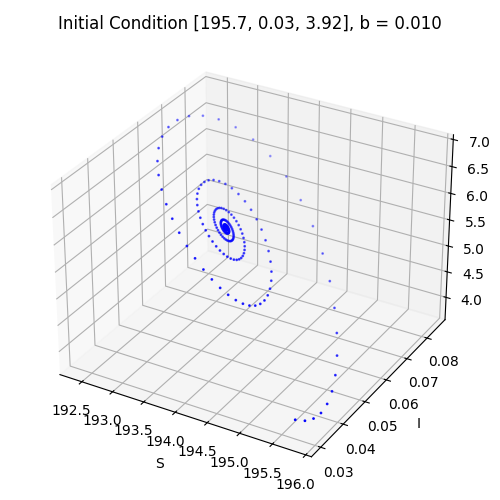
\includegraphics[width=\textwidth]{images/task5/ex4_t5_2_b_1.png}
    \label{fig:subfig_b1}
\end{subfigure}
\begin{subfigure}[b]{0.3\textwidth}
    \centering
    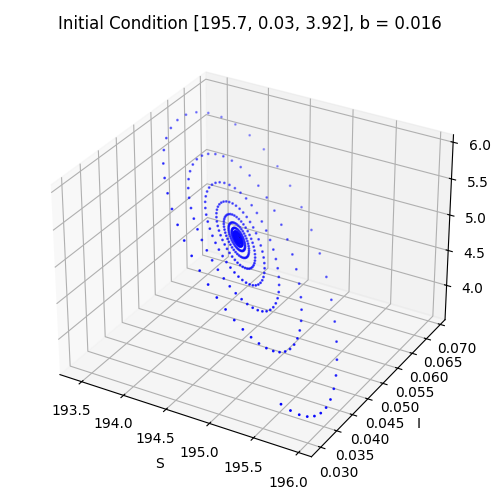
\includegraphics[width=\textwidth]{images/task5/ex4_t5_2_b_7.png}
    \label{fig:subfig_b7}
\end{subfigure}
\begin{subfigure}[b]{0.3\textwidth}
    \centering
    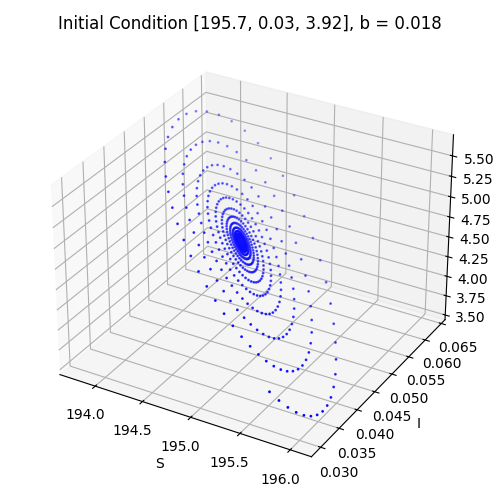
\includegraphics[width=\textwidth]{images/task5/ex4_t5_2_b_9.png}
    \label{fig:subfig_b9}
\end{subfigure}
\begin{subfigure}[b]{0.3\textwidth}
    \centering
    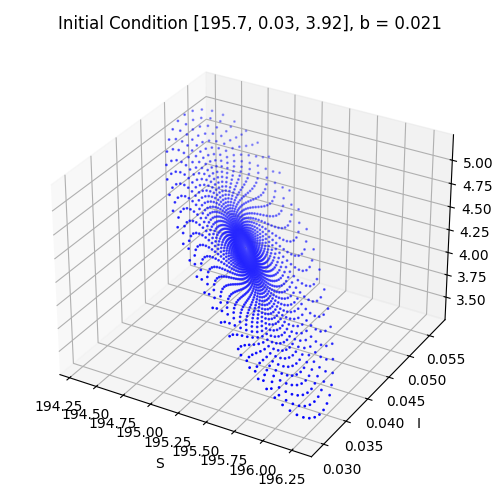
\includegraphics[width=\textwidth]{images/task5/ex4_t5_2_b_12.png}
    \label{fig:subfig_b12}
\end{subfigure}
\begin{subfigure}[b]{0.3\textwidth}
    \centering
    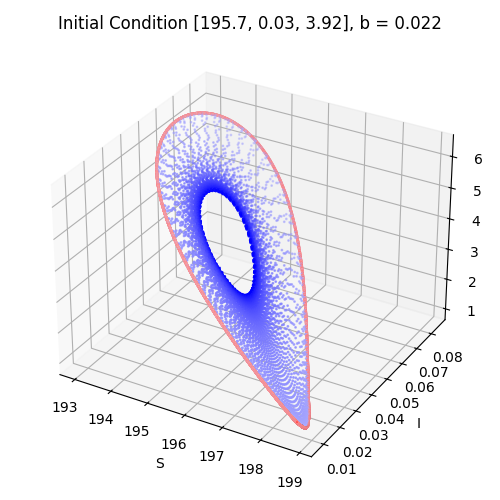
\includegraphics[width=\textwidth]{images/task5/ex4_t5_2_b_13.png}
    \label{fig:subfig_b13}
\end{subfigure}
\begin{subfigure}[b]{0.3\textwidth}
    \centering
    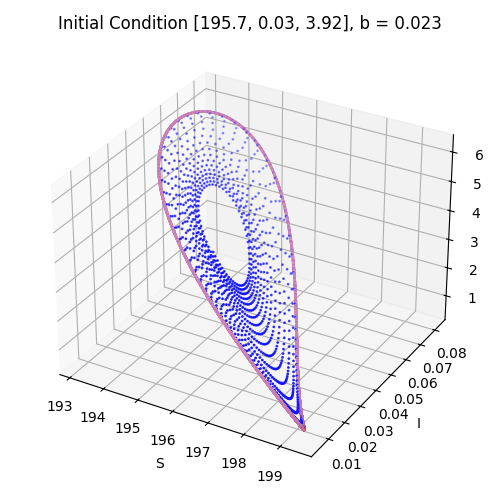
\includegraphics[width=\textwidth]{images/task5/ex4_t5_2_b_14.png}
    \label{fig:subfig_b14}
\end{subfigure}

\begin{subfigure}[b]{0.3\textwidth}
    \centering
    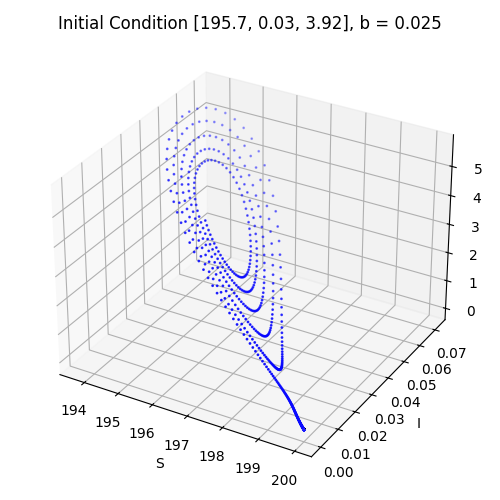
\includegraphics[width=\textwidth]{images/task5/ex4_t5_2_b_16.png}
    \label{fig:subfig_b16}
\end{subfigure}
\begin{subfigure}[b]{0.3\textwidth}
    \centering
    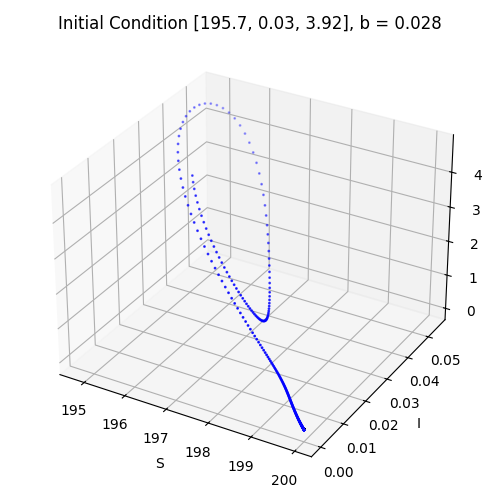
\includegraphics[width=\textwidth]{images/task5/ex4_t5_2_b_19.png}
    \label{fig:subfig_b19}
\end{subfigure}
\begin{subfigure}[b]{0.3\textwidth}
    \centering
    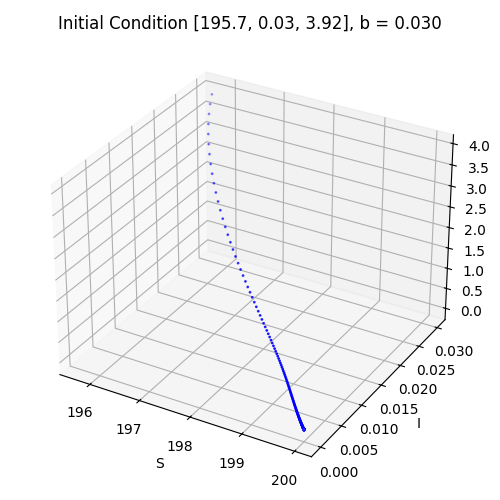
\includegraphics[width=\textwidth]{images/task5/ex4_t5_2_b_21.png}
    \label{fig:subfig_b21}
\end{subfigure}
\caption{State (195.7, 0.03, 3.92) results}
\label{fig:task5_3}
\end{figure}

\item \textbf{Part 4: Bifurcation between b = 0.02 and b = 0.03}

% A series of simulations were conducted on a three-dimensional SIR model, varying the initial conditions to observe the system's behavior over time. 
% The initial conditions were taken from a predefined list, with each entry representing the starting number of susceptible (S), infected (I), and removed (R) individuals, respectively. The parameter \(b\) was fixed at 0.022 for all simulations. The integration over time was performed using the \texttt{solve\_ivp} function from SciPy's integrate module, with a dense output over a specified time grid for high-resolution plots.

% Each simulation's result was visualized in a 3D phase space, with axes corresponding to the S, I, and R variables. The trajectory of the disease spread was depicted using a scatter plot, where the color of each point indicated the time, transitioning from blue (early times) to red (later times). This approach allowed for the identification of the system's behavior under different initial conditions, highlighting any periodic or quasi-periodic patterns, attractors, or bifurcations in the disease dynamics.

Looking at the plots from the previous task, we have already seen that a hopf bifurcation occurs at value of \textbf{b=0.022.}

% To find the exact parameter value of b, at which the Hopf bifurcation occurs, we analyzed the system's equations and identified when the real part of a pair of complex conjugate eigenvalues becomes zero. So the result is 0.022. 

% What bifurcation is that?
\begin{figure}[H]
\centering
\begin{subfigure}[b]{0.3\textwidth}
    \centering
    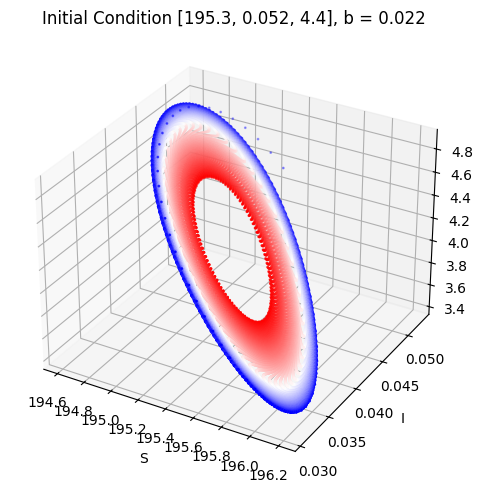
\includegraphics[width=\textwidth]{images/task5/ex4_t5_4_1.png}
    \label{fig:subfig_c1}
\end{subfigure}
\begin{subfigure}[b]{0.3\textwidth}
    \centering
    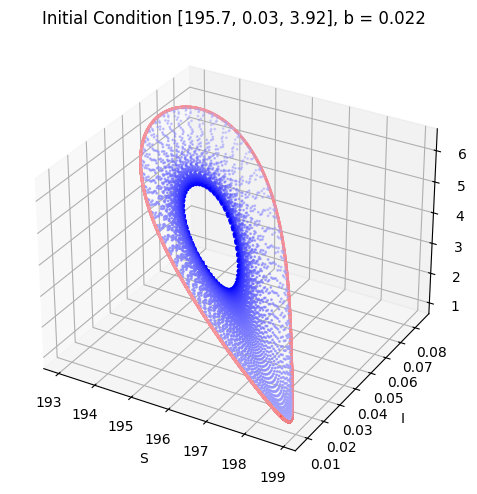
\includegraphics[width=\textwidth]{images/task5/ex4_t5_4_2.png}
    \label{fig:subfig_c2}
\end{subfigure}
\begin{subfigure}[b]{0.3\textwidth}
    \centering
    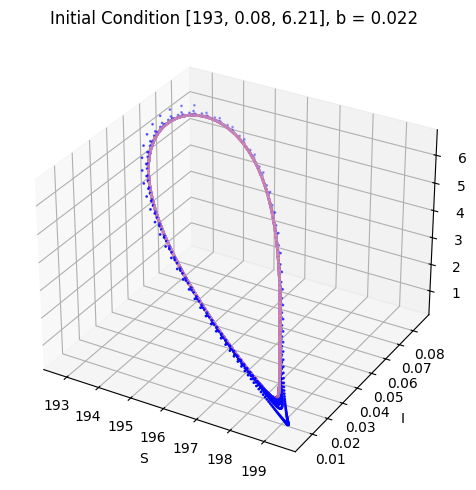
\includegraphics[width=\textwidth]{images/task5/ex4_t5_4_3.png}
    \label{fig:subfig_c3}
\end{subfigure}
\caption{State results}
\label{fig:task5_4_1}
\end{figure}

These images in figure \ref{fig:task5_4_1} show that the system is exhibiting a Hopf bifurcation. A Hopf bifurcation occurs in a dynamical system when a pair of complex conjugate eigenvalues of the linearization around a steady state pass through the imaginary axis in the complex plane. As a result, a limit cycle is created or destroyed, depending on whether the bifurcation is supercritical or subcritical.

The first image shows a closed orbit, which is characteristic of a periodic solution or limit cycle. 
The second image shows a denser set of points forming a torus, suggesting quasi-periodic behavior on a two-dimensional torus.
The third image also shows a closed orbit but with a different shape and size, indicating a change in the system's dynamics.

The normal form of Hopf bifurcation is the same as in specified in the task 3 which can be represented by these equations.

\begin{align*}
    \dot{x_1} = \alpha x_1 - x_2 - x_1(x_{1}^{2}+x_{2}^{2}) \\
    \dot{x_2} = x_1 + \alpha x_2 - x_2(x_{1}^{2}+x_{2}^{2})
\end{align*}

% \begin{equation}
%     \dot{z} = (\lambda + i\omega)z + \alpha |z|^2 z
% \end{equation}

where \( z \) is a complex variable, \( \lambda \) represents the bifurcation parameter, \( \omega \) is the frequency of oscillations, and \( \alpha \) is a complex constant determining the nature and stability of the bifurcation.


% \begin{figure}[H]
%     \centering
%     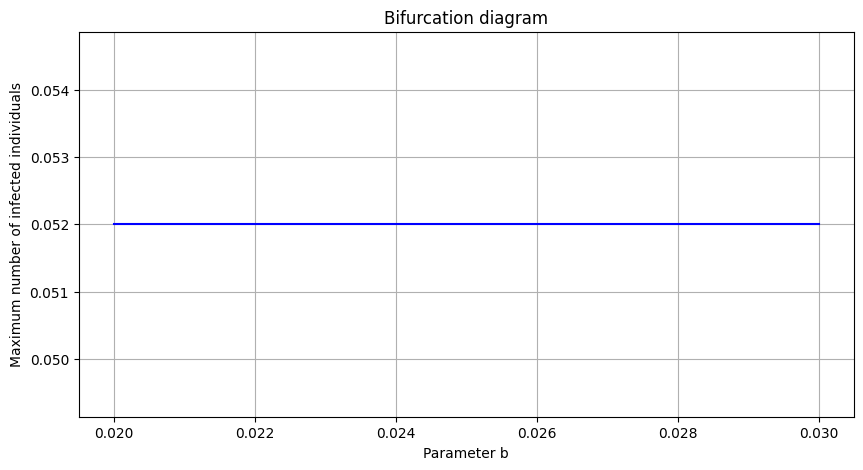
\includegraphics[width=0.8\textwidth]{images/task5/ex4_t5_4_4.png}
%     \caption{Population dynamics over time}
%     \label{fig:task5_4_2}
% \end{figure}

%%% What is the normal form of it? At what parameter value of b does it happen exactly (to three decimal places)


    
\item \textbf{Part 5: Reproduction rate R\_0 }
% Describe which variables are used to compute the reproduction rate...
% ... and what it means for the number of infective persons.

In the paper, the reproduction rate \( R_0 \) is defined in equation (3.1) as follows:

\[
R_0 = \frac{\beta}{d + \nu + \mu_1}
\]
Here, \( \beta \) represents the average number of adequate contacts per unit of time with infectious individuals, \( d \) is the per capita natural death rate, \( \nu \) is the per capita disease-induced death rate, and \( \mu_1 \) is the maximum per capita recovery rate due to sufficient healthcare resources and the inherent property of a specific disease.

When the parameter \( \beta \) increases, it implies more frequent contacts that can potentially lead to infection, thus increasing the reproduction rate \( R_0 \). A higher \( R_0 \) means that each infected person is likely to infect more people, leading to a more rapid spread of the infection. Conversely, if \( \beta \) decreases, it leads to fewer contacts and a lower reproduction rate \( R_0 \), reducing the spread of the infection.

The relationship between the transmission rate \( \beta \) and the reproduction rate \( R_0 \) is visually represented in Figure \ref{fig:reproduction_rate}, where it can be observed that as \( \beta \) increases, so does \( R_0 \). The critical threshold for \( R_0 \) is depicted as a horizontal line at \( R_0 = 1 \), below which the disease is expected to die out, and above which an epidemic can occur.

\begin{figure}[H]
\centering
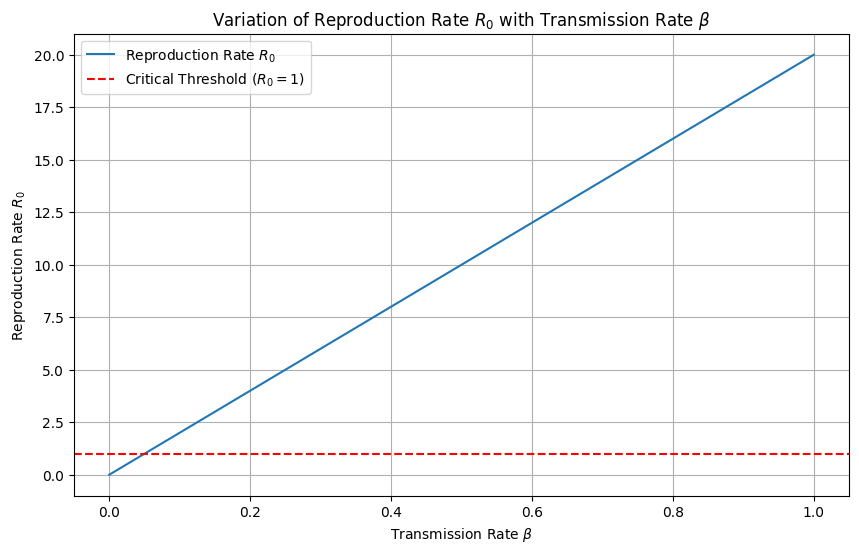
\includegraphics[width=0.8\textwidth]{images/task5/ex4_t5_5_1.png}
\caption{Variation of Reproduction Rate \( R_0 \) with Transmission Rate \( \beta \). The solid blue line represents the reproduction rate as a function of \( \beta \), and the dashed red line indicates the critical threshold where \( R_0 = 1 \).}
\label{fig:reproduction_rate}
\end{figure}

Furthermore, the bifurcation diagram in Figure \ref{fig:bifurcation_diagram} illustrates the existence of an endemic equilibrium when \( R_0 > 1 \), which is possible for higher values of \( \beta \). The blue line indicates that for \( \beta \) values below a critical point, there is no endemic equilibrium and the disease-free state is stable, as shown by the black dot.

\begin{figure}[H]
\centering
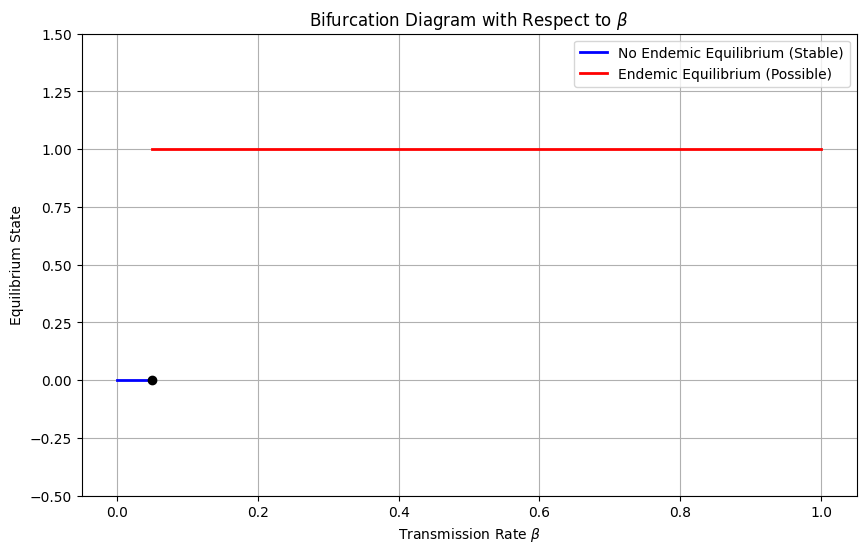
\includegraphics[width=0.8\textwidth]{images/task5/ex4_t5_5_2.png}
\caption{Bifurcation Diagram with respect to \( \beta \). The solid red line shows the range of \( \beta \) values for which the endemic equilibrium exists, and the blue line and dot represent the disease-free equilibrium state.}
\label{fig:bifurcation_diagram}
\end{figure}


\item \textbf{Part 6:  Attractive node}

% What does E0 being an attractive node mean?
% What happens for values of (S, I, R) close to E0?
The behavior described by Theorem 3.2 \cite{Shan_Zhu_2014} is confirmed by the numerical simulations depicted in Figure \ref{fig:task5_6}. As shown, regardless of initial conditions, the trajectories for susceptible (S), infected (I), and recovered (R) individuals converge to the disease-free equilibrium \( E_0 \), which is indicated by the grey dashed line. This convergence is consistent with the theorem's assertion that \( E_0 \) is an attracting node for \( R_0 < 1 \).

\begin{figure}[H]
\centering
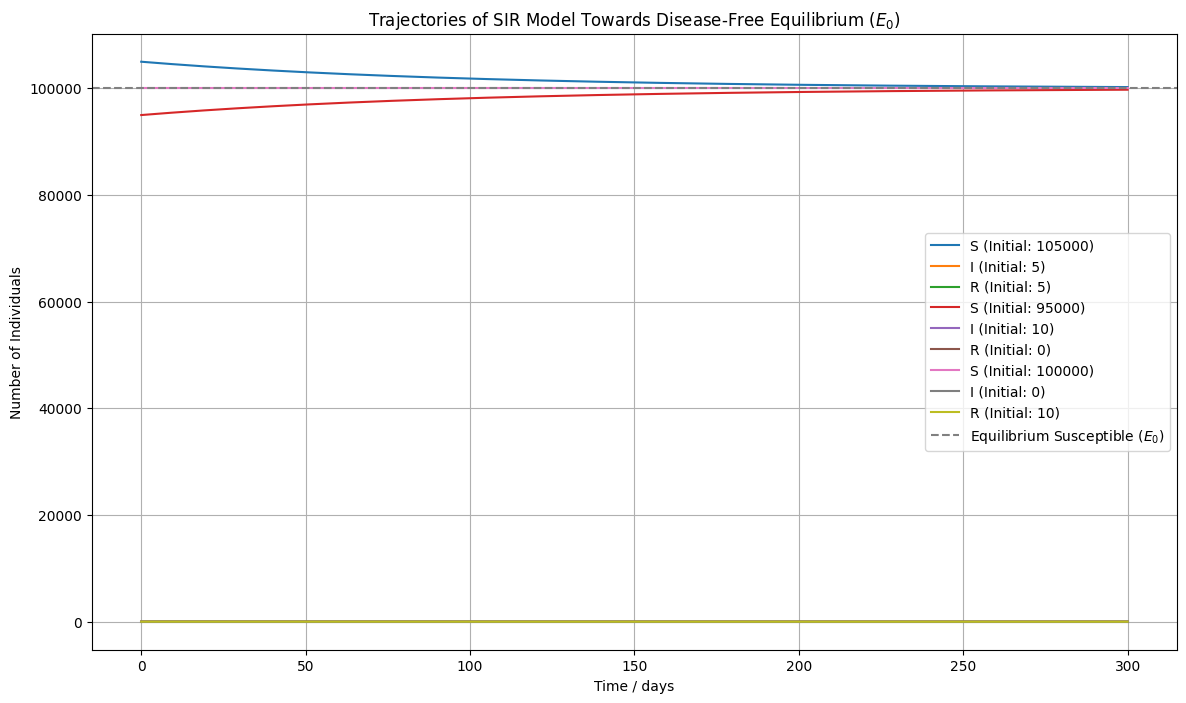
\includegraphics[width=0.8\textwidth]{images/task5/ex4_t5_6.png} 
\caption{Trajectories of SIR Model Towards Disease-Free Equilibrium (\( E_0 \)). The convergence of the trajectories to \( E_0 \) for different initial conditions illustrates that the equilibrium is an attracting node, following Theorem 3.2.}
\label{fig:task5_6}
\end{figure}


\item \textbf{Part 7: Bonus }

%discuss another type of bifurcation model illustration visualization
% Short description of the setup in the report?
Backward bifurcation is a type of bifurcation in which an endemic equilibrium point exists even when the basic reproduction number $R_0$ is less than 1. Usually, this means, that the disease will die out. However, for backward bifurcation, the disease can persist in the population. \\

To implement backward bifurcation, we created the function \texttt{model\_with\_backward\_bifurcation}. The function almost looks the same as the previously used \texttt{model} function. The only difference occurs in the calculation of the variable \texttt{dIdt}. We add a backward bifurcation term: $epsilon * I ** 2$. 
Epsilon is an additional parameter the function takes which should be set to a small positive number. Since the term only depends on epsilon and I, the difference between Hopf bifurcation and backward bifurcation becomes visible once these parameters, especially I, are big enough. In figure \ref{fig:4-5-hb-comparison}, we used $I = 0.52$ and $epsilon = 0.01$. 

\begin{figure}[H]
    \centering
    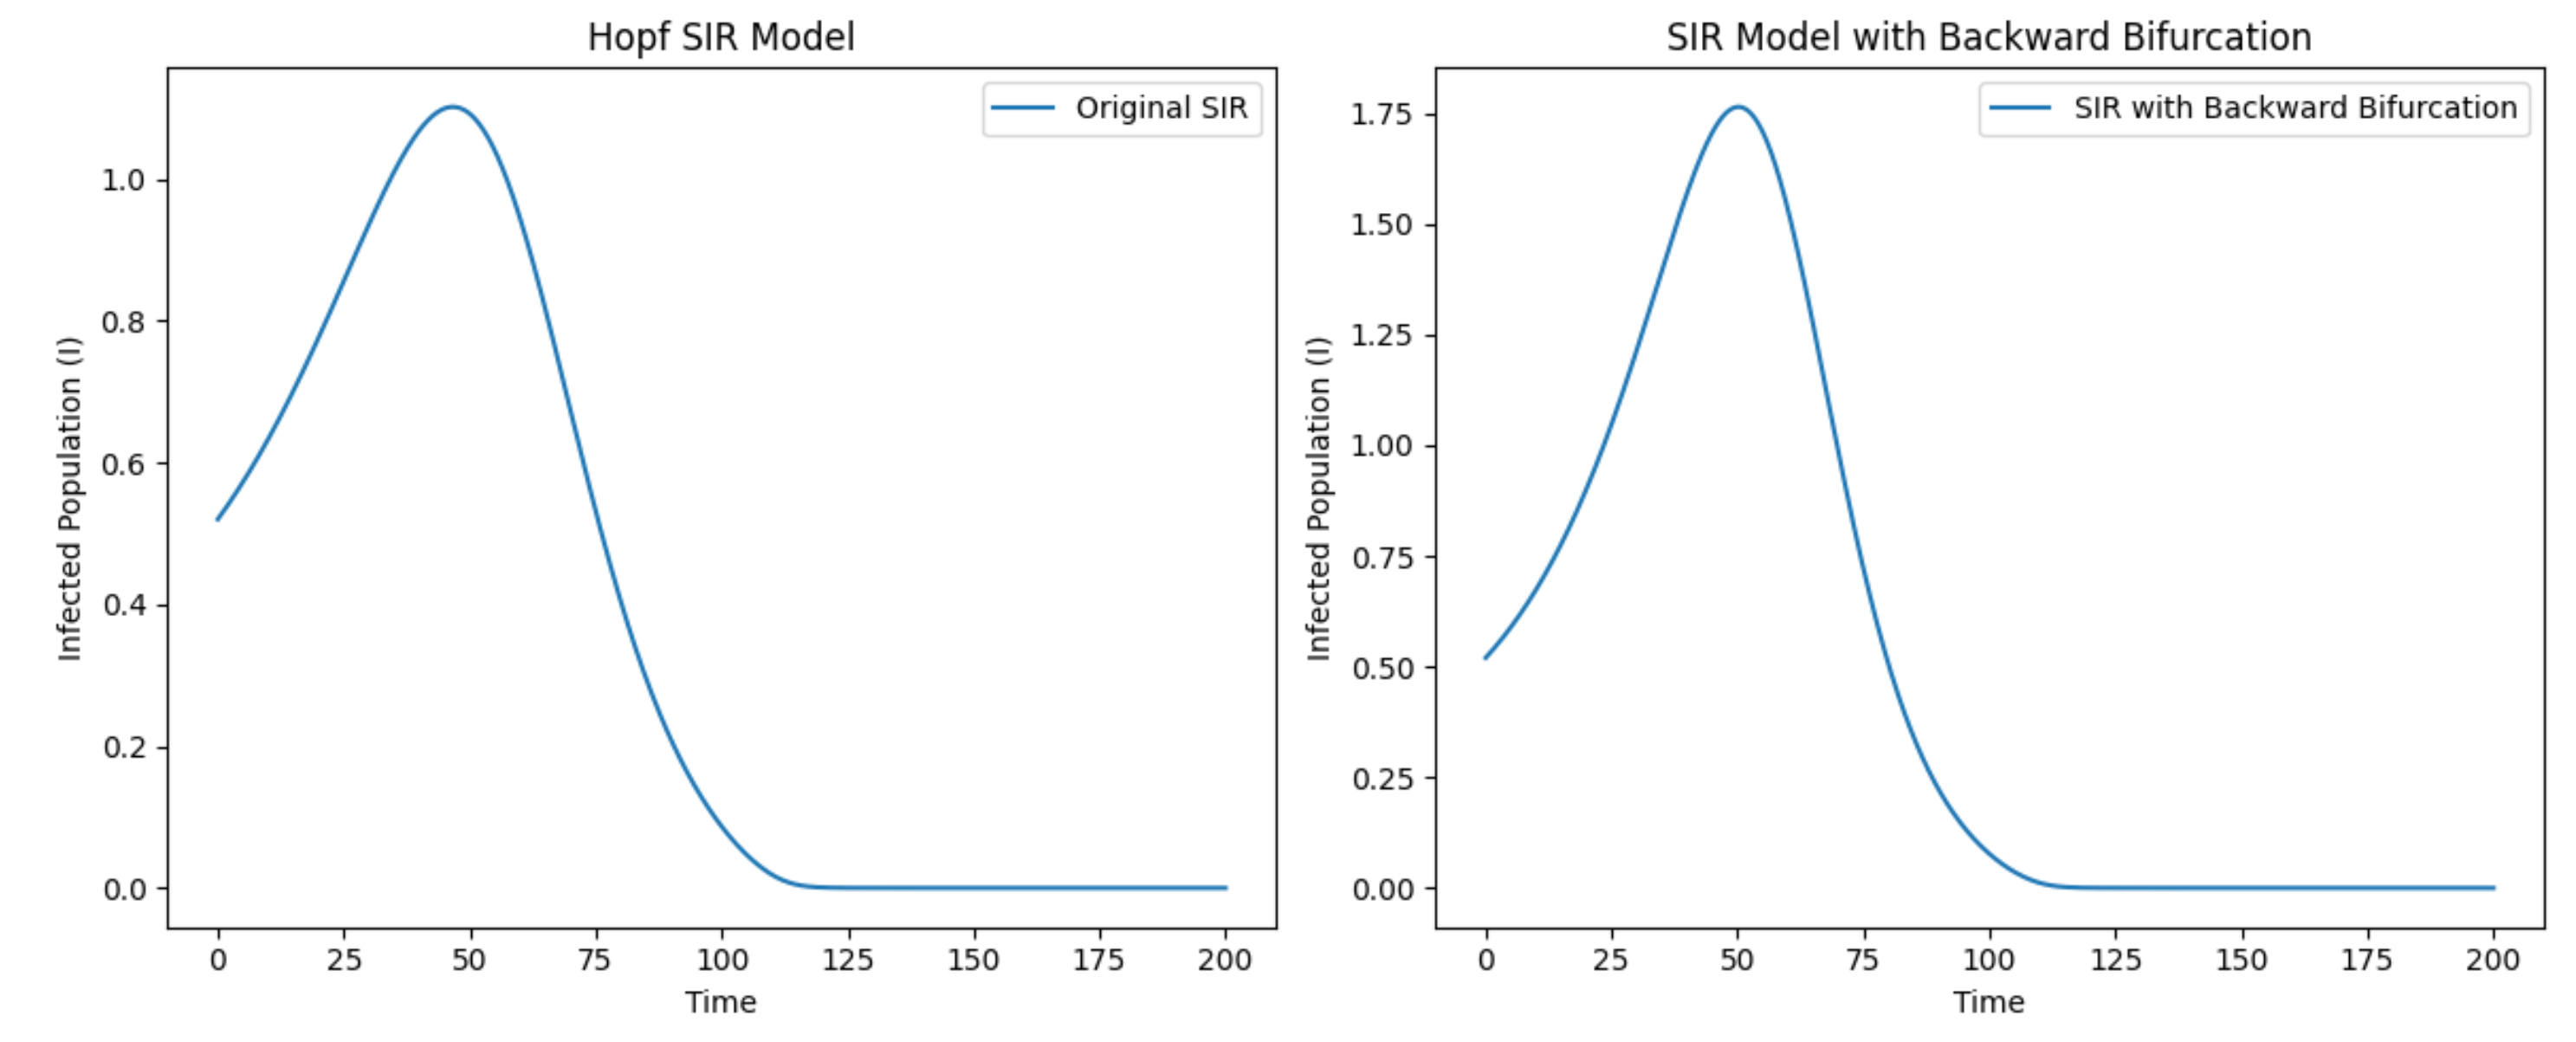
\includegraphics[width=\textwidth]{images/task5/4-5-Hopf-Backward-Comparison.png}
    \caption{Comparison of the Hopf and backward bifurcation models}
    \label{fig:4-5-hb-comparison}
\end{figure}

For the Hopf SIR Model, a nearly constant increase in the infected population can be seen with a maximum at time step 50 of about $I = 1.1$. The value afterward declines until it reaches zero at time step 112. 
In comparison, the backward bifurcation model shows a slight exponential increase up to a maximum of $I = 1.75$ just a bit after time step 50. Despite a higher maximum, the model seems to reach a value of zero four time steps earlier. 

The behavior observed in the backward bifurcation model highlights the complex dynamics of disease transmission and control. It underscores the importance of considering non-linear effects in epidemiological modeling, particularly for diseases with atypical transmission characteristics. The choice of model parameters, including \( \epsilon \), should be informed by the specific disease dynamics and empirical data.
\end{itemize}